\begin{frame}
	\setbeamercolor{block body}{bg = yellow}
	\begin{block}{}
		\begin{center}
			{\large\textbf{Corso di base JAVA}}\\
			\itshape{Mauro Donadeo}\\
			mail: mauro.donadeo@gmail.com
		\end{center}
	\end{block}
	\setbeamercolor{block body}{bg = white}
	\begin{block}{}	
		\begin{center}
			\large{Scrivere i nostri primi programmi}\\
			
\includegraphics[width = 30mm]{images/java-logo.jpg}
		\end{center}
	\end{block}	
\end{frame}

\begin{frame}
\frametitle{Introduzione}
\begin{block}{Cosa tratteremo}
In questa parte tenteremo di andare un po' più a fondo scrivendo diversi programmi e tenteremo di capire
alcune parti specifiche del Java. Alcune cose sono specifiche del linguaggio Java, ma la maggior parte 
sono comuni a tutti i linguaggi di programmazione.
\end{block}
\end{frame}

\section*{Variabili}
\subsection*{Assegnamento}
\begin{frame}
\begin{block}{Le Variabili}
\begin{itemize}
\item Ogni programma fa uso di variabili;
\item le \textbf{variabili} sono spazi di memoria, identificati da un \textbf{nome}, che possono contenere \textbf{valori}
di qualsiasi tipo
\item ciascuna variabile deve essere \textbf{definita}, indicandone il \alert{tipo} ed il \textCl{nome};
\item Una variabile può contenere soltanto valori dello \textbf{stesso tipo}.
\item Nella definizione di una variabile è possibile \textCl{assegnarle} un \alert{valore iniziale}.
\end{itemize}
\end{block}
\end{frame}

\begin{frame}[fragile]
\begin{block}{}
Supponiamo di avere un conto corrente con all'interno 50.00 euro. E che riceveremo un acconto per un lavoro di 500.00 euro.
\end{block}
\pause
\begin{lstlisting}
amountCount = 50.00;
amountCount = amountCount + 500.00;
\end{lstlisting}
\begin{block}{}
Nel pezzo di codice sopra viene fatto uso di \texttt{amountCount} che è una \textit{variabile}. E questa variabile viene
inizializzata con $50.00$. Questo numero potrà variare, naturalmente il vecchio valore non verrà memorizzato.
\end{block}
\end{frame}

\subsection*{Tipi di variabile}
\begin{frame}
\begin{block}{}
Quando si pensa ad un computer che memorizza una lettera ad esempio la lettera J esso in realtà memorizza la sequenza 
\texttt{01001010}, ogni cosa all'interno di un computer è una sequenza di 0 e 1, più comunemente sequenze di \textCl{bit}.
\end{block}
\begin{block}{01001010}
Questa sequenza inoltre può assumere altri significati:
\begin{itemize}
\item Come detto precedentemente la lettera J
\item ma anche il numero intero 74;
\item $1.036960863003646 x 10^{-43}$
\end{itemize}
\end{block}
\begin{block}{}
\textit{Il computer distingue il tipo della sequenza utilizzando il concetto di \textCl{tipo}}. Il tipo di una variabile è
il range di valori che può assumere.
\end{block}
\end{frame}

\begin{frame}[fragile]
\begin{lstlisting}
import static java.lang.System.out;
class acconto {
   public static void main(String args[]) {
       double amountAccount = 50.00;
       amountAccount = amountAccount + 500.00;
       out.print("You have:");
       out.print(amountAccount);
       out.println(" in your account.");
   }	
}
\end{lstlisting}
\begin{block}{}
\texttt{double ammountAccount;}
Indica la \textit{dichiarazione di una variabile}. Nella dichiarazione della variabile la parola \texttt{double} è 
una \textit{keyword} Java.
\end{block}
\end{frame}

\subsection*{I tipi primitivi di Java}
\begin{frame}
\begin{block}{}
La parola \texttt{double} è un esempio di tipo primitivo in Java (anche come conosciuti \textit{tipi semplici}).
\end{block}
\begin{table}[h]\footnotesize
\begin{tabular}{c c c}
\toprule
\multicolumn{3}{c}{Tipi primitivi di Java}\\
\cmidrule(r){1-3}
\textbf{Tipo} & \textbf{Che valore rappresentano} & \textbf{Range di valori}\\
\hline
\texttt{byte} & \texttt{(byte)42} & -128 a 127 \\
\hline
\texttt{short} & \texttt{(short)42} & -32768 a 32767 \\
\hline
\texttt{int} & \texttt{42} & –2147483648 a \\ 
 & & 2147483647\\
\hline
\texttt{long} & \texttt{42L} & –9223372036854775808 a\\
& & 9223372036854775807\\
\hline
\texttt{float} & \texttt{42.0F} & $-3.4x10^{38} a 3.4x10^{38}$\\
\hline
\texttt{double} & \texttt{42.0} & $-1.8x10^{308} a 1.8x10^{308}$\\
\hline
\texttt{char} & \texttt{'A'} & Centinaia di caratteri, simboli \\
\hline
\texttt{boolean} & \texttt{true} & true, false\\
\bottomrule
\end{tabular}
\end{table}
\end{frame}

\subsection*{Creare nuovi valori utilizzando gli operatori}
\begin{frame}
\frametitle{Cosa si può fare con l'operatore \alert{+}}
\begin{block}{Classico}\footnotesize
\texttt{\textCl{int}} mele, pere, frutta;\\
\texttt{mele = 5;}\\
\texttt{pere = 10;}\\
\texttt{frutta = mele + pere;}\\
\end{block}
\pause
\begin{block}{Concatenazione}\footnotesize
\texttt{String concatenazione = ``Questa è la prima stringa ''\textCl{+} ``Questa è la seconda stringa''}\\
E' possibile anche concatenare stringhe con numeri\\
\texttt{System.out.println(``Tu hai comprato: ''\textCl{+} frutta \textCl{+}`` pezzi di frutta'');}
\end{block}
\pause
\begin{block}{Operatori}
Chiaramente valgono tutti gli altri operatori aritmetici che possiamo immaginare: \textCl{- * / \%}
\end{block}
\end{frame}

\begin{frame}
\begin{block}{Operatori di incremento e decremento}
\begin{itemize}
\item \texttt{nomeVariabile++/nomeVariabile--} incrementa/decrementa di una unità il valore della variabile dopo averla valutata;
\item \texttt{++nomeVariabile/--nomeVariabile} incrementa/decrementa la variabile di una unità prima che essa venga valutata.
\end{itemize}
\end{block}
\begin{block}{Assignment operators}
E' possibile anche effettuare un incremento maggiore di uno: per esempio sommare due o cinque o 100000.
\begin{itemize}
\item \texttt{numberIncrement += 1;} La variabile viene incrementata di uno;
\item \texttt{numberIncrement +=10000;} La variabile viene incrementata di 10000;
\item \texttt{numberIncrement *= 500;} La variabile viene moltiplicata per 500;
\end{itemize}
\end{block}
\end{frame}

\section*{Oggetti, classi, metodi}
\begin{frame}
\begin{block}{}
\begin{huge}
\large{\begin{center}
\textCl{Oggetti, classi, metodi}
\end{center}}
\end{huge}
\end{block}
\end{frame}
\subsection*{Oggetti}
\begin{frame}
\frametitle{Oggetti}
\begin{block}{}
Un \textbf{oggetto} è un'entità che può essere manipolata in un programma mediante l'invocazione dei suoi \textbf{metodi}
\end{block}
\begin{columns}
\begin{column}{0.5\textwidth}
\begin{block}{}
\begin{itemize}
\item \textCl{pippo} è un oggetto;
\item appartiene alla classe \textbf{String}
\item si può manipolare ad esempio mediante i suoi \textCl{metodi}
\begin{itemize}
\item ad esempio \textbf{toUppercase}
\end{itemize}
\end{itemize}
\end{block}
\end{column}
\begin{column}{0.5\textwidth}
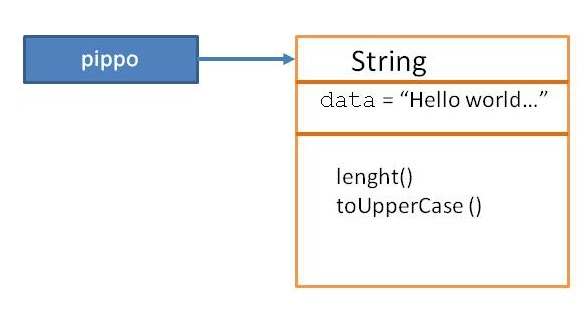
\includegraphics[scale=0.4]{images/classe.jpg}
\end{column}
\end{columns}
\begin{block}{}\footnotesize
Per il momento consideriamo un oggetto come una \textbf{black box} dotata di una \textbf{interfaccia pubblica}, che definisce il comportamento dell'oggetto, e una sua realizzazione \textbf{nascosta} (il codice dei metodi ed i loro dati)
\end{block}
\end{frame}

\subsection*{Classi}
\begin{frame}
\begin{block}{Una classe}
\begin{itemize}
\item è una \textbf{fabbrica di oggetti};
\begin{itemize}
\item gli oggetti che si creano sono \alert{esemplari}
\end{itemize}
\item specifica i metodi che si possono invocare per gli oggetti che sono esemplari di tale classe.
\item definisce i particolari della realizzazione dei metodi
\item è un contenitore di :
\begin{itemize}
\item metodi statici;
\item oggetti statici;
\end{itemize}
\end{itemize}
\end{block}
\end{frame}

\subsection*{Metodi}
\begin{frame}
\begin{block}{}
Costituiscono l'\textCl{interfaccia pubblica} di una classe:
\begin{itemize}
\item Istruzioni valide:
\begin{itemize}
\item \texttt{String pippo = ``Hello world'';}
\item \texttt{int n = pippo.\alert{lenght()};}
\item \texttt{String river = ``Missisipi'';}
\item \texttt{String BigRiver = river.\alert{toUpperCase();}}
\end{itemize}
\item Istruzione non valida (il metodo non appartiene alla classe):
\begin{itemize}
\item \texttt{System.out\alert{.lenght();}}
\end{itemize}
\end{itemize}
\end{block}
\end{frame}

\begin{frame}
\frametitle{Metodi, parametri espliciti/impliciti}
\begin{block}{}
Alcuni metodi necessitano di \textCl{valori in ingresso} che specificano l'operazione da svolgere.
\begin{center}
\texttt{System.out.printf(\textCl{pippo})}
\end{center}
\textCl{pippo} in questo caso rappresenta un parametro esplicito.
\end{block}
\begin{block}{}
Altri metodi invece non necessitano di alcun parametro. Tutte le informazioni sono memorizzate nell'oggetto corrispondente.
\begin{center}
\texttt{int n = \textCl{pippo}.length();}
\end{center}
\textCl{pippo} in questo caso è il parametro implicito.
\end{block}
\end{frame}

\begin{frame}
\frametitle{Definizione dei metodi}
\begin{block}{}
\textbf{public} \alert{void} \textCl{println(String output)}
\textbf{public} \alert{String} \textCl{replace(String target,String replace)}
\end{block}
\begin{block}{}
La \textbf{definizione di un metodo} inizia sempre con la sua \textbf{intestazione}, composta da:
\begin{itemize}
\item uno specificare di accesso:
\begin{itemize}
\item in questo caso è \textbf{public}, ma esiste anche la clusula \textbf{private};
\end{itemize}
\item il tipo di dati restituito dal metodo (\alert{Sting, void, int, double\ldots}
\item il nome del metodo (\textCl{println, replace, length})
\item un elenco di parametri, eventualmente vuoto, chiuso tra \textCl{parentesi tonde}
\begin{itemize}
\item di ogni parametro si indica il tipo e nome
\item più parametri sono separati da una virgola.s
\end{itemize}
\end{itemize}
\end{block}
\end{frame}

\begin{frame}
\frametitle{Variabili oggetto}
\begin{block}{}
Una \textCl{variabile oggetto} conserva non l'oggetto stesso, ma informazioni sulla sua posizione nella memoria del computer.
Sostanzialmente è un \alert{riferimento} all'oggetto.
\end{block}
\begin{block}{}
Per definire una variabile oggetto si indica il nome della \textbf{classe} a cui l'oggetto farà riferimento la variabile,
seguito dal nome della \textCl{variabile} stessa.
\begin{center}
\alert{NomeClasse} \textCl{nomeOggetto}
\end{center}
\end{block}
\begin{block}{}
La definizione di una variabile oggetto crea un riferimento \textbf{non inizializzato}, cioè la variabile non fa riferimento ad 
alcun oggetto.
\end{block}
\end{frame}

\begin{frame}
\frametitle{Costruire oggetti: l'operatore new}
\begin{block}{}
Per \textbf{creare un oggetto} di una classe si usa l'operatore \textCl{new} seguito dal \alert{nome della classe} e da una coppia
di parentesi tonde
\begin{center}
\texttt{\textCl{new} \alert{NomeClasse}(parametri)}
\end{center}
\end{block}
\begin{block}{}
L'operatore \textCl{new} \textbf{crea un nuovo oggetto e ne restituisce un riferimento, che può essere assegnato ad una variabile}
del tipo appropiato.
\begin{center}
\textbf{NomeClasse} \alert{nomeVar} = \textCl{new} \textbf{NomeClasse(parametri)}
\end{center}
\end{block}
\end{frame}

\begin{frame}
\frametitle{ESERCIZIO}
\begin{block}{}
Creare un rettangolo descritte dalle coordinate (x,y) del suo vertice in alto a sinistra e dalla larghezza e altezza.
\end{block}
\begin{block}{}
Creare un secondo rettangolo con le stesse caratteristiche del primo, e successivamente traslarlo di (15,20).
\end{block}
\begin{block}{}
Stampare le caratteristiche sia del primo che del secondo rettangolo.
\end{block}
\begin{block}{}
Potete importare la classe Rectangle, presente nel pacchetto in \alert{java.awt.Rectangle}
\end{block}
\end{frame}

\begin{frame}
\frametitle{Programmi di controllo}
Sono utilizzati per collaudare il funzionamento di una classe.
\begin{itemize}
\item Definire una nuova classe;
\item Definire in essa un nuovo metodo main;
\item Costruire oggetti all'interno del metodo main;
\item Applicare metodi agli oggetti
\item Visualizzare i risultati delle invocazioni dei metodi.
\end{itemize}
\alert bisogna importare le classi che si vuole utilizzare.

\begin{block}{}
Tutte le classi della libreria standard sono raccolte in \textbf{pacchetti} e sono organizzate in pacchetto o finalità. 
\texttt{java.lang} (al quale appartengono \textbf{System} e \textbf{String}) viene importata automaticamente.
\end{block}

\end{frame}